\documentclass[main]{subfiles}

\begin{document}

\chapter{Manual de usuario}
\label{chap:anexo_manual}

Este manual de usuario indica los pasos a seguir para volar el cuadric\'optero en modo hovering. Se asume que la IMU se encuentra previamente calibrada. 

\section{Montaje y conexionado}

\subsubsection{Componentes del sistema}
Montar sobre la plataforma los distintos componentes del sistema:
\begin{itemize}
\item BeagleBoard, BeagleJuice y m\'odulo de WiFi en la caja de acr\'ilico como se detalla en el cap\'itulo \ref{chap:montaje}.
\item IMU
\item ESC
\item GPS
\item Placa de conversi\'on de niveles l\'ogicos
\item Bater\'ia
\end{itemize}
Si se desea habilitar la opci\'on de utilizar el control remoto debe incluirse la CPU de f\'abrica, el receptor y el circuito encargado del switcheo (ver cap\'itulo \ref{chap:anexo_switcheo}).

\subsubsection{Conexiones}
En esta secci\'on se detallan las conexiones de los componentes.
\begin{itemize}
\item Conexiones de la BeagleBoard
	\begin{itemize}
	\item Alimentar la BeagleBoard con 5v provenientes de la BeagleJuice.
	\item Conectar en un puerto USB el módulo de WiFi, en otro el GPS y en un tercero un pendrive.
	\item Conectar con la placa de conversión de niveles lógicos, bas\'andose en los nombres de las se\~nales indicados sobre la placa, y la p\'agina 108 del BeagleBoard-xM System Reference Manual.
	\end{itemize}
\item Conexiones de la IMU
	\begin{itemize}
	\item Conectar la alimentaci\'on (5V) a la BeagleJuice.
	\item Conectar las señales de Gnd, 3.3V, Tx y Rx a la placa de conversión de niveles l\'ogicos.
	\end{itemize}
\item Conexión de los ESCs
	\begin{itemize}
	\item Conectar las lineas del $I^2C$ (SDA, SCLK, GND) a la placa de conversión de niveles l\'ogicos.
	\item Conectar a los motores. En la figura \ref{fig:conexion_motores} puede observarse la correspondencia entre ESC y motores.
	\item Conectar la bater\'ia
	\end{itemize}
\end{itemize}

En caso de desearse utilizar también el control remoto, conectar la CPU de f\'abrica y el circuito de Switcheo de acuerdo a las conexiones que se especif\'ican en el cap\'itulo \ref{chap:anexo_switcheo}.

\begin{figure}
	\centering
	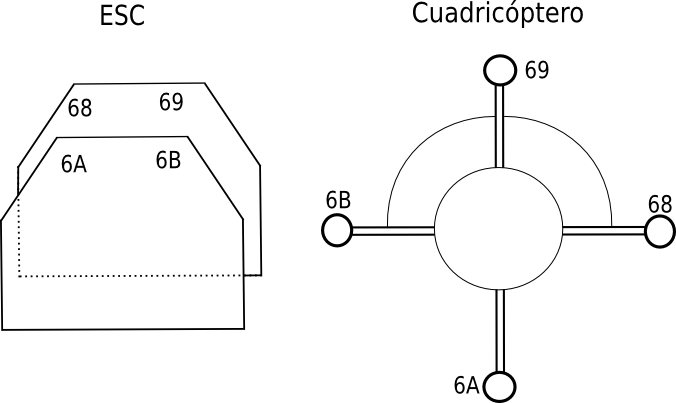
\includegraphics[width=0.7\textwidth]{./pics_manual/diagrama.png}
	\caption{Correspondencia entre motores y ESC}
	\label{fig:conexion_motores}
\end{figure}

Se debe hacer coincidir el plano de la IMU con el plano formado por los motores de acuerdo al procedimiento explicado en el cap\'iutlo \ref{chap:montaje}. Para mostrar en consola las lecturas de la IMU en deben ejecutarse los siguiente comandos:
\begin{quote}
\begin{verbatim}
ssh root@10.42.43.2
cd work/uquad/src/build/test/imu_comm_test
./imu_comm_test /dev/ttyS1
\end{verbatim}
\end{quote}

Las columnas 10 a 12 indican los \'angulos de Euler. Se deben ajustar los tornillos de la IMU hasta que dichos \'angulos sean lo m\'as cercano posible al cero.

\section{Ajuste del Offset}

Para resolver el problema del offset se ejectura el driver de los motores y se le env\'ian comando desde la consola, hasta lograr equilibrar el \'angulo en cuesti\'on. Para correr el driver ejecutar los siguientes comandos:

\begin{quote}
\begin{verbatim}
ssh root@10.42.43.2
cd work/uquad/src/i2c_beagle
make stdin
./cmdstdin X69 X6A X6B X68
\end{verbatim}
\end{quote}

Cada uno de los par\'ametros \verb+X6M+ puede ser \verb+1+ o \verb+0+: El \verb+1+ habilita el motor \verb+6M+, y el \verb+0+ lo deshabilita.

\begin{itemize}
\item Offset del \'angulo de Yaw
	\begin{enumerate}
	\item Colgar el cuadric\'optero de forma que pueda girar respecto al eje vertical. 
	\item Ejecutar
          \begin{equation*}
            \verb+./cmdstdin 1 1 1 1+
          \end{equation*}
          a una velocidad de $I^2C$ lo m\'as alta posible sin que el cuadric\'optero se levante (Se sugiere utilizar 120 $I^2C$ trabajando con un peso de aproximadamente 1.7kg).
	\item Ajustar los offsets en la consola, enviando distintos valores hasta que el cuadric\'optero no gire, y luego escribir el resultado en
          \begin{equation*}
            \verb+src/i2c_beagle/cmd_motores.c+
          \end{equation*}
          para que sea tomado en cuenta siempre que se compile el driver.
	\end{enumerate}
\item Offset del \'angulo de Pitch y de Roll: Los ajustes en estos \'angulos no deber\'ian modificar mucho el offset encontrado para el Yaw, ya que el torque neto no se modifica. De cualquier forma, puede cambiar el punto de operaci\'on y por lo tanto afectar al Yaw.
	\begin{enumerate}
	\item Ubicar el cuadric\'optero de forma que tenga libre un solo eje de giro.
	\item Para el Pitch ejecutar:
          \begin{equation*}
            \verb+./cmdstdin 1 1 0 0+
          \end{equation*}
          Igual que en el caso anterior ajustar el offset de forma que el cuadric\'optero se mantenga horizontal.
	\item Repetir para el Roll ejecutando:
          \begin{equation*}
            \verb+./cmdstdin 0 0 1 1+
          \end{equation*}
	\end{enumerate}	
      \item Revisar los tres \'angulos para verificar los offsets obtenidos.
\end{itemize}

\section{Pruebas del Controlador}
\begin{itemize}
\item Prueba de los \'angulos de Roll y de Pitch
	\begin{enumerate}
	\item Ubicar el cuadric\'optero de forma que tenga libre un solo eje de giro posible.
        \item Modificar las matrices \verb+K_prop_full_ppzt.txt+ y \verb+K_int_full_ppzt.txt+ de forma que las unicas entradas distintas de cero sean las que corresponden a la realimentaci\'on del \'angulo de inter\'es, de la velocidad angular de inter\'es y de la integral del error del \'angulo de inter\'es. Las matrices de realimentaci\'on se encuentran en \verb+src/control+.
        \item Modificar el driver \verb+src/i2c_beagle/cmd_motores.c+, ya que por defecto prender todos los motores. Descomentar las l\'ineas que inhabilitan los motores que no se van a utilizar (buscar cerca de la l\'inea 697).
	\item Correr el loop de control (\verb+./go.sh+), modificar dichas matrices hasta encontrarse conforme con la respuesta del sistema. Partir de los valores dados por el algoritmo LQR en MatLab.
	\item Repetir con el otro \'angulo (cambiar nuevamente las matrices y el driver).
	\end{enumerate}
\item Prueba del \'angulo de Yaw.
	\begin{enumerate}
	\item Colgar el cuadric\'optero.
	\item Setear la Masa del cuadric\'optero lo m\'as alto posible sin que el cuadric\'optero levante vuelo (se sugiere utilizar 1.4Kg si el cuadric\'optero levanta vuelo con 1.7kg).
	\item Modificar las matrices \verb+K_prop_full_ppzt.txt+ y \verb+K_int_full_ppzt.txt+ hasta lograr el comportamiento deseado. Partir de los valores dados por el algoritmo LQR.
	\end{enumerate}
\end{itemize}
Una vez realizadas las pruebas anteriores el cuadric\'optero deber\'ia presentar un comportamiento estable. De todas formas se sugiere agregar dos cuerdas de seguridad: una por encima y otra por debajo, de forma de limitar el movimiento del mismo y evitar accidentes. Tener especial con las cuerdas, en caso de enredarse con un motor cortar la ejecuci\'on de inmediato para evitar da\~nar ESCs o motores.\\

\textbf{NOTA:} Los ESCs disponibles presentan un problema conocido como FOD\footnote{Flip Of Death} que hace que alguno de los motores deje de funcionar. Es un evento aleatorio, respecto a cuando sucede y respecto a el motor que afecta. Evitar hacer pruebas muy largas o muchas pruebas consecutivas para reducir los riesgos\footnote{No fue comprobado que esto evite el FOD.}.
\end{document}